\documentclass[11pt]{amsart}
\usepackage{geometry}                % See geometry.pdf to learn the layout options. There are lots.
\geometry{letterpaper}                   % ... or a4paper or a5paper or ... 
%\geometry{landscape}                % Activate for for rotated page geometry
%\usepackage[parfill]{parskip}    % Activate to begin paragraphs with an empty line rather than an indent
\usepackage{graphicx}
\usepackage{amssymb}
\usepackage{epstopdf}
\DeclareGraphicsRule{.tif}{png}{.png}{`convert #1 `dirname #1`/`basename #1 .tif`.png}

\title{Lumped Parameter Model for Bear Spring}
\author{Huang, Kang, Langevin}
%\date{}                                           % Activate to display a given date or no date

\begin{document}
\maketitle

In karst regions, springs provide a focused outflow point for groundwater discharge.  A simple lumped parameter model is developed here to approximate the relationship between recharge, spring discharge, and changes in aquifer storage.  The conceptual model is shown in Figure \ref{fig:concept}.    

\begin{figure}[!ht]
	\begin{center}
	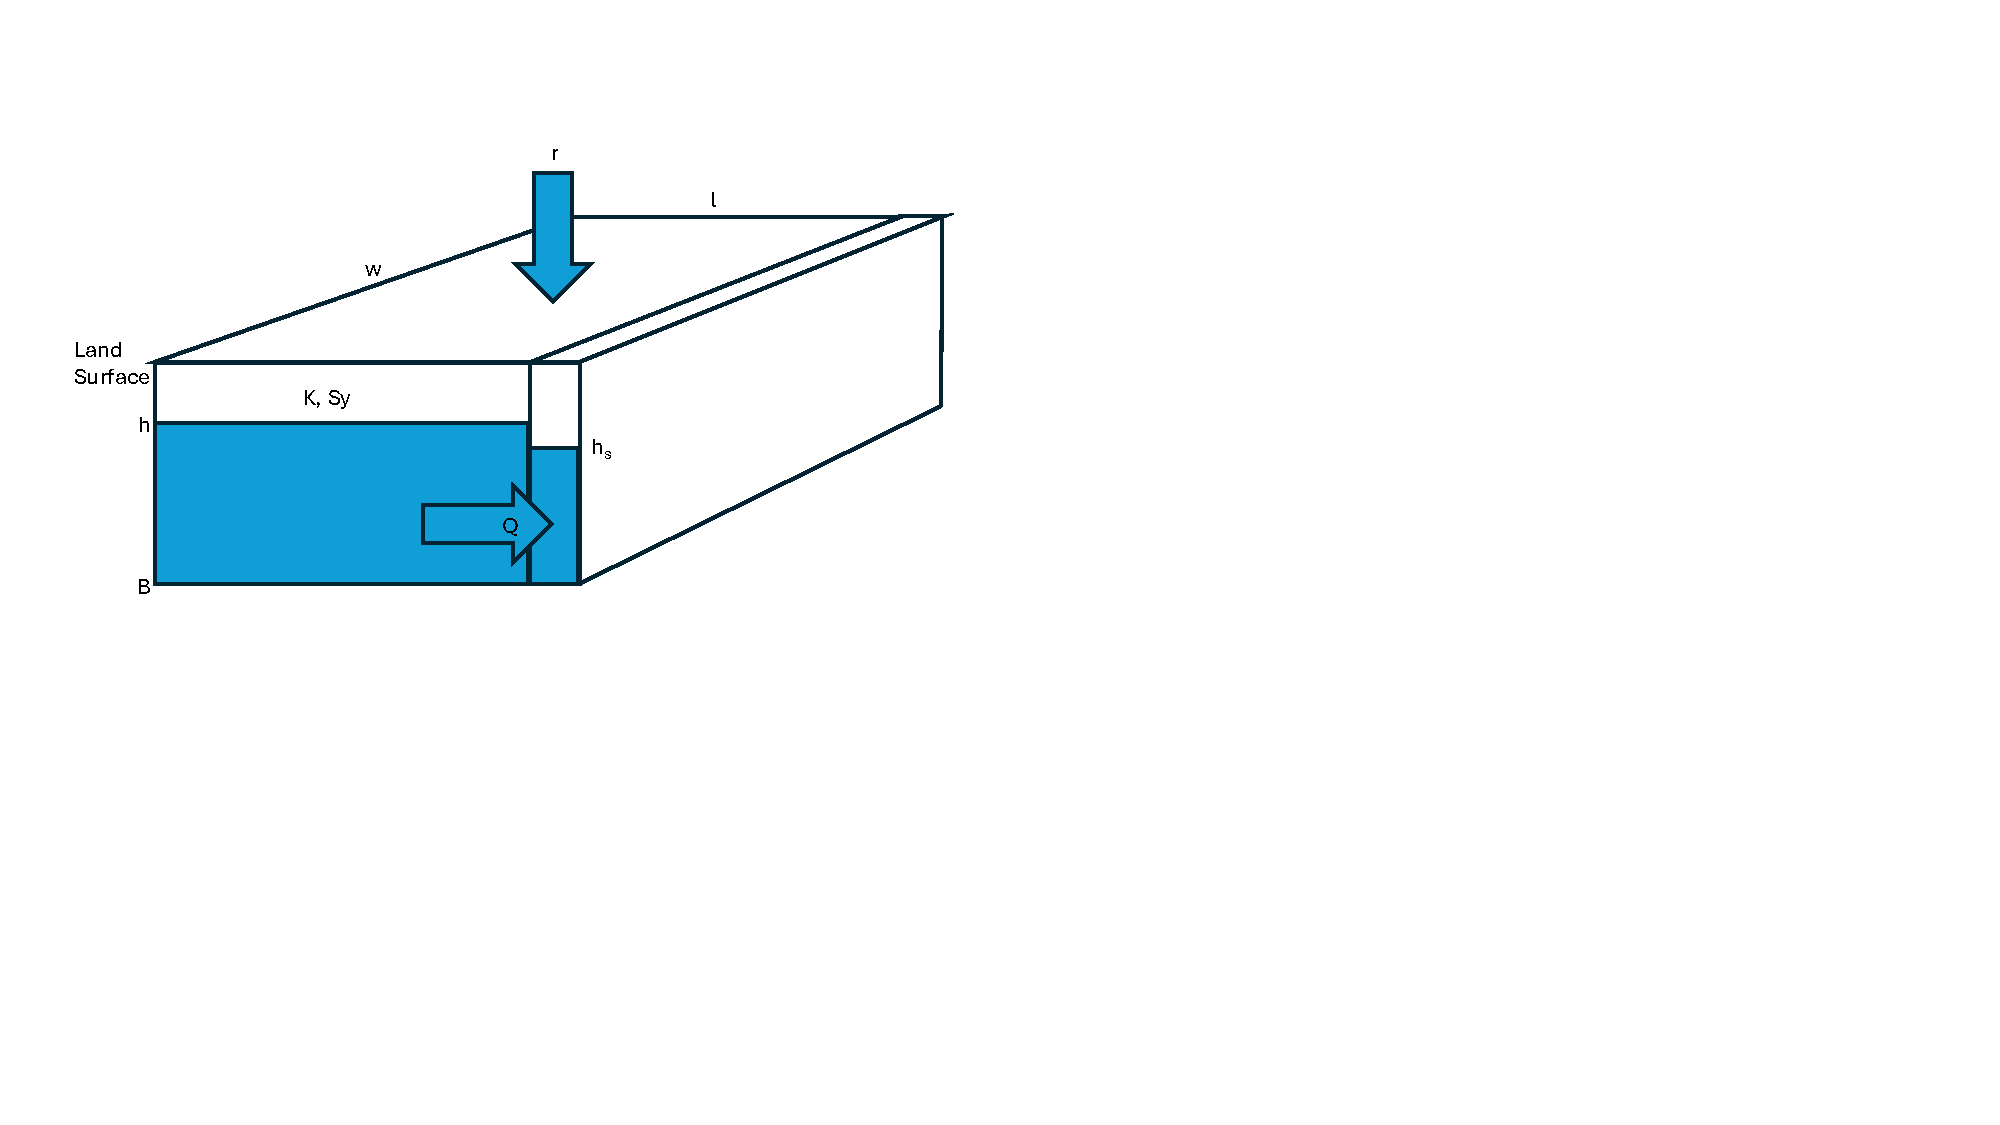
\includegraphics[width=1.0\textwidth]{./concept.pdf}
	\caption[capt]{text}
	\label{fig:concept}
	\end{center}
\end{figure}

In this simple conceptual model, a linear spring feature is connected on one side of an unconfined aquifer. The elevation of the spring stage is specified as $h_s$.  The aquifer has dimensions of $w$ by $l$, giving the plan-view area of the spring shed ($A_s$) as $l \times w$.  The elevation of the water table is given by $h$, which is assumed to be uniform over the entire area.  Land surface bounds the top of the aquifer; the bottom of the aquifer is assumed to be flat at an elevation of $B$.  It would be possible to route any water above land surface to the spring as overland flow, however this is not included yet.

Recharge falls on the spring shed at a uniform rate of $r$ length units per time.  Groundwater discharge to spring is denoted by $Q$ and has dimensions of length cubed per time.  A simple balance equation for such a system is expressed as, 

\begin{equation}
I - O = \Delta S,
\end{equation}

\noindent where $I$ is the sum of all inflow, $O$ is the sum of all outflows, and $\Delta S$ is the change in storage.  For the case considered here, inflow to the spring shed, in dimensions of length cubed per time, is expressed as $r A_s$.  Outflow occurs through groundwater discharge to the spring ($Q_s$) , expressed as:

\begin{equation}
Q_s = C \left ( h_s - h \right ),
\end{equation}

\noindent where $C$ is the conductance in length squared per time.  $C$ can be expressed in a variety of different ways.  One simple way is assign it as

\begin{equation}
C = \frac{2 \overline{K} w b}{l}.
\end{equation}

\noindent which is a Darcy-based approach assuming an average flow distance of half the $l$ value.  $\overline{K}$ is used here to denote an average hydraulic conductivity over the height of the aquifer in contact with the spring.  It may be possible to use a calculated value for $\overline{K}$ as a function of $h$ to allow it to vary as individual preferential pathways are activated.  The $b$ term represents the height of the aquifer in contact with the spring.  It can be assigned as a constant, or it could be calculated from the aquifer and spring head using some form of averaging.

The storage term, $\Delta S$ can be expressed as

\begin{equation}
\Delta S = A_s S_y \left ( \frac{h^{t + \Delta t} - h^t}{\Delta t} \right )
\end{equation}

From these equations, we can write an explicit solution for $h^{t + \Delta t}$ and march through time to calculate head and spring discharge as a function of recharge, spring shed geometry, and aquifer properties.



%\section{}
%\subsection{}



\end{document}  